% !TeX program = lualatex
% !TeX encoding = UTF-8
% !TeX spellcheck = fr_FR

\documentclass[a4paper, french, twoside]{article}
\usepackage{polyglossia}
\setdefaultlanguage{french}
\usepackage{fontspec}
\defaultfontfeatures{Ligatures={Common, TeX}}
\usepackage[pdfusetitle, colorlinks=true]{hyperref}
\usepackage{mathtools, amssymb}
\usepackage{xcolor}
\usepackage{graphicx}
\usepackage[left=2cm, right=2cm, top=2cm, bottom=2cm]{geometry}
\usepackage{subcaption}
\captionsetup[sub]{subrefformat =brace}
\usepackage{multicol}
\usepackage{dsfont}
\usepackage{enumitem}
\setlist{noitemsep}
\usepackage{float}
\definecolor{airforceblue}{rgb}{0.36, 0.54, 0.66}
\graphicspath{{C:/Users/Adrien Dubois/Desktop/TIPE/2-Code/images/}}
	
\title{Application de méthodes de recherche d'isomorphismes de graphes à la comparaison des structures de protéines}
\author{Adrien Dubois - N° Candidat : 51771}
\date{\today}

\begin{document}
\maketitle
\tableofcontents

\vfill

\section{Contexte, données à traiter et objectif}
\subsection{Contexte, objectif}
La compétition Casp est un concours de prédiction informatique de structures de protéines à partir de séquences d'acides aminés.
Les modèles proposés sont déjà connus, il faut alors comparer les structures informatiques et expérimentales.
Un moyen de comparaison permettrait d'affiner la précision des prédictions et ainsi remplacer les méthodes de détermination experimentales longues et coûteuses
par des méthodes informatiques. \newline
\hspace*{0.4cm} Finalement, la structure d'une protéine permet une meilleure compréhension de la protéine; par exemple est nécessaire pour la fabrication de médicaments.

\begin{center}
\begin{tabular}{ccc}
    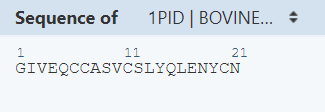
\includegraphics[width=3cm]{sequence_insuline_bovine}
    & 
    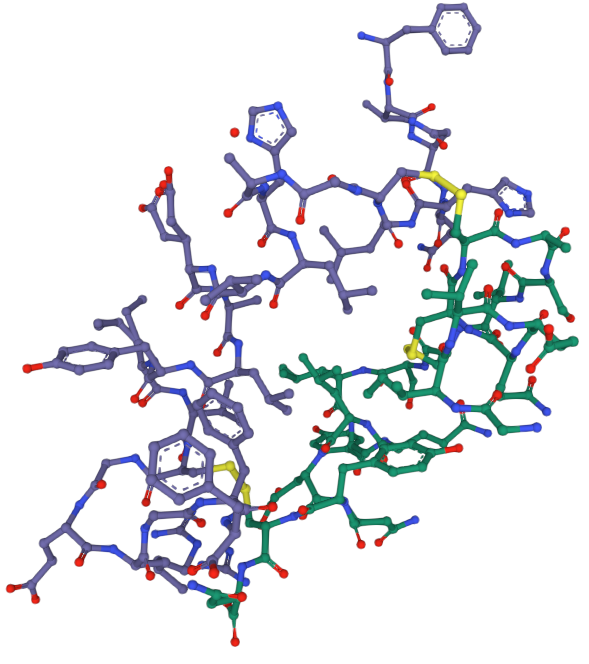
\includegraphics[width=2cm]{structure_insuline_bovine}
    &
    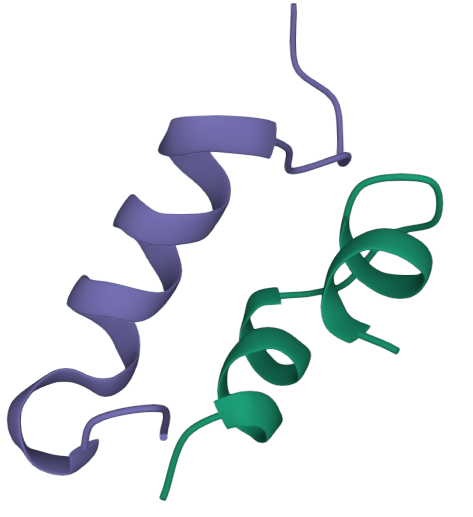
\includegraphics[width=2cm]{cartoon_insuline_bovine} \\
    \textit{Séquence} & \textit{Structure} & \textit{Représentation simplifiée}
\end{tabular}
\end{center}
source : Protein Data Bank, https://www.rcsb.org/3d-view/1B0Q \cite{pdb} \newline

\noindent \underline{Objectif} : proposer une méthode de comparaison de structures

\subsection{Format PDB \cite{pdb}}
Voci un fichier PDB :

\begin{figure}[!htb]
    \centering
    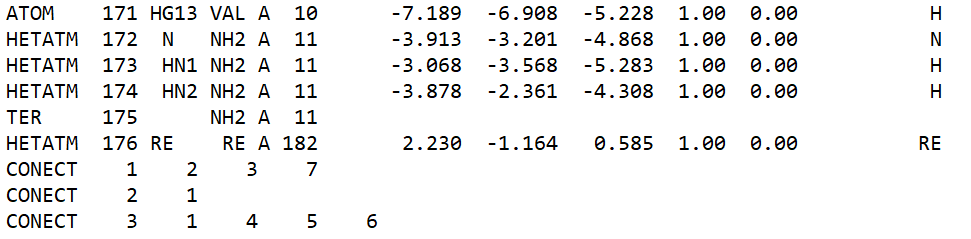
\includegraphics[width=9cm]{lignes_pdb}
    \caption{\label{fig:fichier_pdb}Lignes d'un fichier PDB}
\end{figure}

A partir de ce fichier on extrait :
\begin{itemize}
    \item les atomes
    \item le type (carbone, hydrogène, etc)
    \item la position dans l'espace des atomes
    \item les liaisons (attention, à cause de considérations biologiques non prises en compte peu de liaisons sont lues)
\end{itemize}
\begin{figure}[!htb]
    \centering
    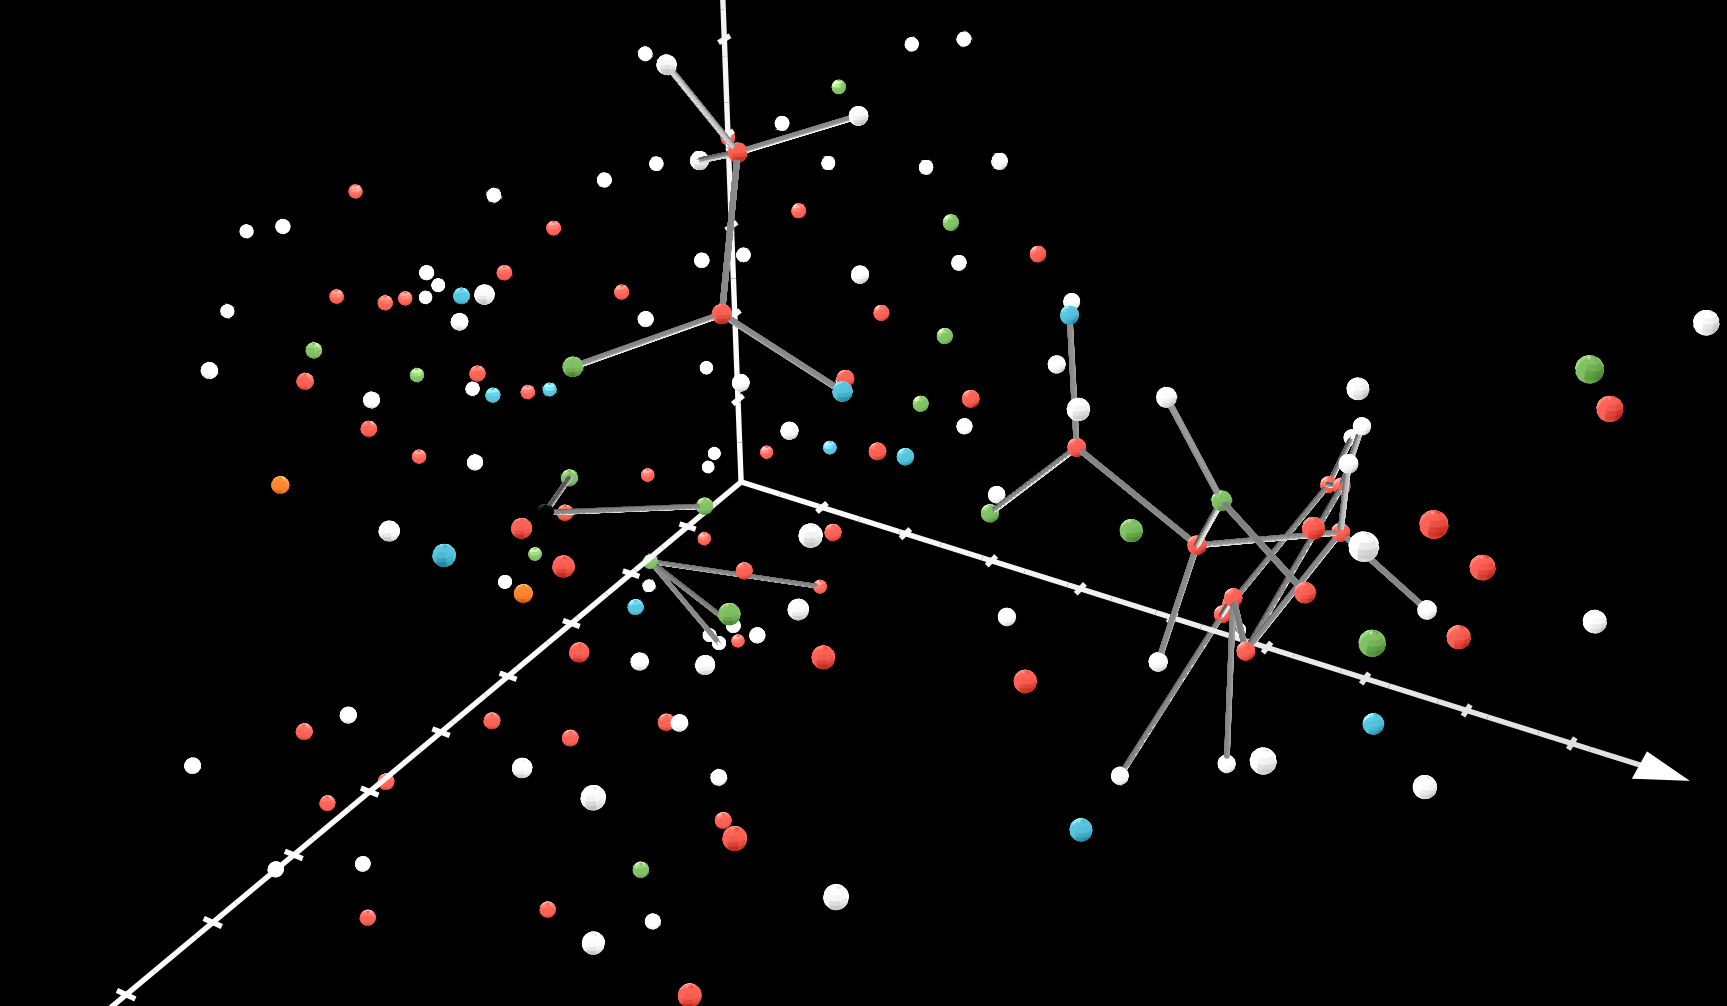
\includegraphics[width=12cm]{protein_peuliaisons_pres}
    \caption{\label{fig:lecture_pdb} Affichage du PDB à l'aide de la bilbiothèque python manim}
\end{figure}

\section{Comparaison de branches (pas de ramifications)}

\subsection{Branche}
Une branche $B_1 = [M_1,\cdots,M_n]$ est une suite de points ordonnés dont les liaisons sont de proche en proche (liaison de $M_1$ à $M_2$, $M_2$ à $M_3$, etc)
\subsection{Coefficient de comparaison}
L'idée est d'associer à deux branches données de même taille un coefficient de proximité R$\in [0,1]$, deux paramètres sont considérés :
\begin{itemize}
    \item l'écart moyen des longueurs des liaisons
    \item les angles que forment deux liaisons situées au même niveau des branches
\end{itemize}
Soit $B_1 = [M_1,\cdots,M_n]$ et $B_2 = [N_1,\cdots,N_n]$ des branches.
On pose $\forall i \in [\![1,n-1]\!]$ :
\begin{equation*}
l_i = M_iM_{i+1},\ l_i' = N_iN_{i+1},\ d_i = max(l_i,l_i'), \text{ et }
\theta_i = angle(  \overrightarrow{M_iM_{i+1}} ,   \overrightarrow{N_iN_{i+1}} ) 
\end{equation*}
\begin{equation*}
    C_{dist} = \frac{\displaystyle\sum_{i=0}^{n-1} | \sin(\frac{\theta_{i}}{2}) | d_i}{\displaystyle\sum_{i=0}^{n-1} d_i} \qquad  
    C_{angle} = \frac{\displaystyle\sum_{i=0}^{n-1} |l_i' - l_i|}{\displaystyle\sum_{i=0}^{n-1} d_i}
\end{equation*}
\begin{equation*}
    R_{dist} = \frac{1}{1 + C_{dist}} \qquad R_{angle} = \frac{1}{1 + C_{angle}}
\end{equation*}
\newline Finalement, on définit : \newline
\begin{equation*}
    \boxed{R = \frac{R_{dist}+R_{angle}}{2}}
\end{equation*}

\subsection{Valeur du coefficient sur des exemples}

\begin{multicols}{2}
    \begin{figure}[H]
        \centering
        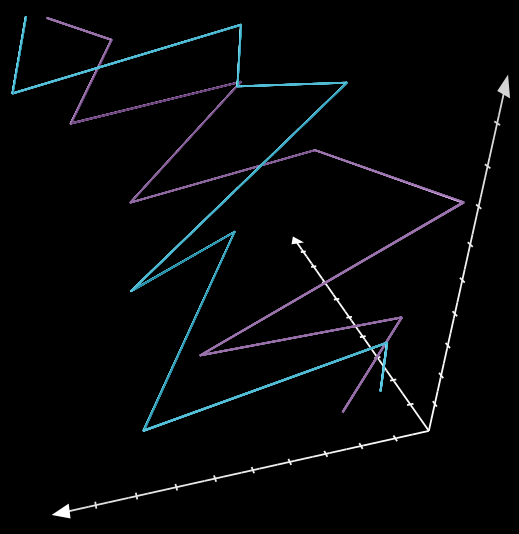
\includegraphics[width=4cm]{rcoeff_dist059_ang068_tot064}
        \caption{\label{fig:branche_a} Branche A}
    \end{figure}
    \vfill
    \begin{figure}[H]
        \centering
        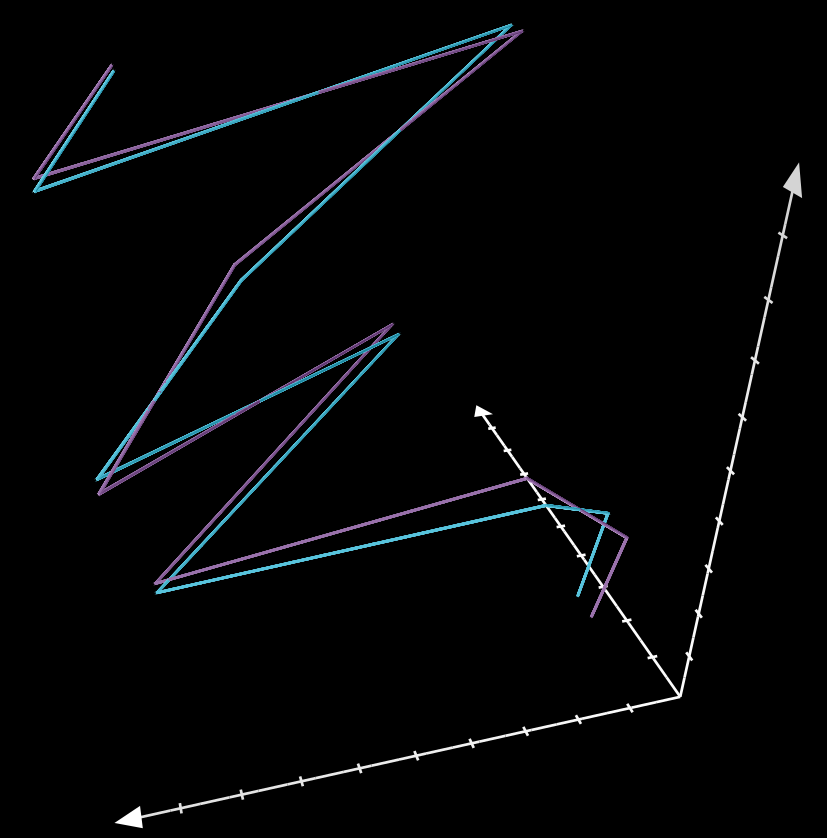
\includegraphics[width=4cm]{rcoeff_dist094_ang097_tot095}
        \caption{\label{fig:branche_b} Branche B}
    \end{figure}
\end{multicols}

\begin{multicols}{2}
    \begin{align*}
        R_{dist} = &0.59 \quad R_{angle} = 0.68 \\
        &\boxed{R = 0.64}
    \end{align*}
    \vfill
    \begin{align*}
        R_{dist} = &0.94 \quad R_{angle} = 0.97 \\
        &\boxed{R = 0.95}
    \end{align*}
\end{multicols}

\section{Isomorphisme de protéines}
\subsection{Isomorphisme de graphes}

\fbox{
\begin{minipage}{0.95\textwidth}
\underline{Définiton} : Soit $A_g$=$\lbrace g_1,\cdots,g_n \rbrace$ et $A_h$=$\lbrace h_1,\cdots,h_n \rbrace$ des ensembles
\newline Soit G=$A_g \times S_g$ et H=$A_h \times S_h$ 
deux graphes où $S_g,S_h\subseteq[n]\times[n]$ 
\newline ( ainsi, l'arête $(g_i,g_j)$ est dans G $\iff (i,j)\in S_g$ ) :
\begin{equation}
G \cong H\ si\ et\ seulement\ si\
\exists \sigma \in \Sigma _n, S_g = S_h^\sigma
\end{equation}
où $S_h^\sigma := \lbrace (\sigma(i),\ \sigma(j)),\ \exists (i,j) \in [\![1,n]\!]^2,\ (i,j) \in S_h \rbrace$
\end{minipage}}

\subsection{Force brute}
Itération sur $n!$ permutations, on test si H permuté est le même graphe que G

\subsection{Tri des sommets par invariants}
\fbox{%
\begin{minipage}{0.95\textwidth}
    On crée une partition de $[\![1,n]\!]$ des sommets $(V_1|\dots| V_t)$ pour G
    et $(W_1|\dots|W_t)$ pour H tels que $\forall i \in [\![1,t]\!]$,
    $V_i=( v_{i,1}\ \dots\ v_{i,|V_i|} )$ et $W_i=( w_{i,1}\ \dots\ w_{i,|W_i|} )$
    alors :
    \begin{align}
        G \cong H \iff
        \exists (\sigma_i)_{i\in[\![ 1,t]\!]} \in 
        \Sigma _{|V_1|}\times..\times\Sigma _{|V_t|},\ 
        G=H^{\sigma} 
        \text{avec } \sigma \ :\
        \left( \begin{array}{ll}
            & \forall j \leq |W_1|,\ w_{1,j} \longmapsto w_{1,\sigma_1(j)} \\
            & \qquad \cdots \\
            & \forall j \leq |W_t|,\ w_{t,j} \longmapsto w_{1,\sigma_t(j)}
        \end{array} \right)
    \end{align}
\end{minipage}}\newline \newline

\underline{Exemple} :
\begin{align*}
    (V_1,V_2) &\to ( \quad 1 \quad 2 \quad 3 \quad| \quad 4 \quad 5\quad ) \\
    (W_1,W_2) &\to ( \quad 1 \quad 3 \quad 5 \quad| \quad 2 \quad 4\quad )
\end{align*}
\begin{center}
\begin{tabular}{cccc}
    $\sigma_1$ 
    \footnote{$pour\ \sigma \in \Sigma_n ,\ on\ note\ \sigma = (\sigma(1)\ \sigma(2)\ \cdots\ \sigma(n)) $}
    & $\sigma_2$ & $(W_1^{\sigma_1}|W_2^{\sigma_2})$ & $\sigma = \tilde{\sigma_1} \circ \tilde{\sigma_2}$ \\
    \hline
    $(1\ 2\ 3)=Id$ & $(1\ 2)=Id$ & $( 1\quad 3\quad 5\ |\ 2\quad 4)$ & $(1\quad 3\quad 5\quad 2\quad 4)$ \\
    $(3\ 2\ 1)$ & $(1\ 2)=Id$ & $( 5\quad 3\quad 1\ |\ 2\quad 4)$ & $(5\quad 3\quad 1\quad 2\quad 4)$ \\
    $(1\ 2\ 3)=Id$ & $(2\ 1)$ & $( 1\quad 3\quad 5\ |\ 4\quad 2)$ & $(1\quad 3\quad 5\quad 4\quad 2)$ \\
\end{tabular}
\end{center}

G et H sont des graphes à n sommets tous deux \textbf{triés canoniquement}:
\begin{itemize}
    \item types des $t \in \mathbb{N}$ paquets du tri sont dans le \textbf{même ordre} 
    \item on suppose les paquets de chacun des tris de \textbf{même taille $t_i,\ i \in [\![1,t]\!]$ deux à deux} (sinon les graphes seraient trivialement non isomorphes)
    \newline 
\end{itemize} 
\begin{center}
\begin{tabular}{ccc}
    & force brute & tri des sommets \\ & & \\
    procédé d'itération & permutations sur $\Sigma_n$ & combinaison de permutations sur \\
    & & $(\Sigma_i)_{i \in [\![1,t]\!]}$ tel que $\sum_{i=1}^t t_i  = n$ \\
    nombre maximal d'itérations & $n!$ & $\prod_{i=1}^t t_i!$ \\
    & & \\
    mise en mémoire nécessaire & $\sum_{k=1}^n k! $ permutations & $\sum_{k=1}^{max(t_1,..,t_t)} k! $ permutations \\
\end{tabular}
\end{center} \normalsize

\section{Isomorphisme canonique de McKay \cite{mckay}}
\begin{tabular}{ll}
\underline{Idée générale}: & $\bullet \quad$ tri équitable des sommets à partir d'un tri \\
& $\quad \rightarrow \quad$ informations avec la propagation du degré \\
& $\quad \rightarrow \quad$ tri optimal \\
& \\
& $\bullet \quad$ création d'un arbre de recherche de permutations \\
& $\quad \rightarrow \quad$ on crée artificiellement de nouveaux tris équitables \\
& $\qquad \quad$ (fils de l'arbre) en isolant des sommets \\
& $\quad \rightarrow \quad$ les feuilles sont des tris ordonnés de parties à un \\ 
& $\qquad \quad$ sommet : ce sont des permutations \\
& $\bullet \quad$ définition d'un ordre total sur les graphes \\
& $\quad \rightarrow \quad$ déterminer le plus grand pour cette relation parmi \\
& $\qquad \quad$ les graphes permutés avec les feuilles de l'arbre \\
& $\quad \rightarrow \quad$ on obtient alors l'\underline{isomorphisme canonique}
\end{tabular}

\subsection{Tri équitable \cite{mckay_label}}
\noindent \underline{Utilisation de la propagation du degré} : \newline \newline 
Tri des sommets des paquets par degré dans les autres paquets pour en faire un nouveau tri,
jusqu'à ce qu'il n'y ait plus de simplification possible \newline \newline
Soit $\pi = (1\ |\ 3\ 7\ 9\ |\ 6\ 8\ |\ 2\ 4\ |\ 5)$ un tri des sommets du graphe G \newline
\hspace*{0.9cm} = $(V_1\ |\ V_2\ |\ V_3 \ | \ V_4\ |\ V_5)$

\begin{figure}[!htb]
    \centering
    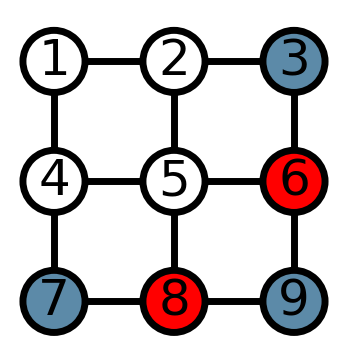
\includegraphics[width = 2.5cm]{graph_tri_equal_colored}
    \caption{\label{fig:graph_tri_colored} Graphe G avec $\textcolor{airforceblue}{V_2} \textcolor{airforceblue}{=(3 \ 7\ 9)}$ et $\textcolor{red}{V_3} \textcolor{red}{=(6\ 8)}$}
\end{figure} 
\begin{center}
    Tri de $V_2$ par degré dans $V_3$ : deg(3,$V_3$)=deg(7,$V_3$)=1 et deg(9,$V_3$)=2 \\
    donc $V_2 = (3\ 7\ |\ 9)$ et $\pi ' = (1\ |\ 3\ 7\ |\ 9\ |\ 6\ 8\ |\ 2\ 4\ |\ 5)$ est plus fin
\end{center}

\noindent underline{Tri équitable} : la propagation de degré ne donne plus de nouveau tri
\begin{align*}
    & \forall (i,j)\in[\![1,n]\!]^2, \text{ tous les sommets de } V_i \text{ ont le même degré dans } V_j \\
    \iff \ & \forall (i,j)\in[\![1,n]\!]^2,\ 
    \forall (v,w) \in V_i^2,\ deg(v,V_j)=deg(w,V_j) \\
\end{align*}
\underline{Relation d'ordre partiel sur les partitions}
Soit $\pi_1 = (V_1|\dots| V_t)$ et $\pi_2=(W_1|\dots| W_{t'})$ des partition de $[\![1,n]\!]$
\begin{equation}
    \text{alors } \pi_1 \text{ est plus fin que } \pi_2 \iff
    \left\{
    \begin{array}{ll}
        & \forall V \in \pi_1, \exists W \in \pi_2,\ V\subseteq W \\
        & \forall i \leq j,\ \forall W_k,W_l,\ (\ V_i\subseteq W_k \text{ et } V_j\subseteq W_l \ \Rightarrow 
        \ k \leq l \ )
    \end{array}
    \right.
\end{equation}

Soit $\pi$ un tri, on note :
\begin{equation}
    \boxed{R(\pi) \text{ le tri équitable ordonné le plus fin obtenu à partir de \pi}}
\end{equation} 

\subsection{Arbre de recherche \cite{mckay_label}}

On considère le tri suivant le degré $\pi = (1\ 3\ 7\ 9\ |\ 2\ 4\ 6\ 8\ |\ 5)$ dans le graphe G (défini ci-dessus). \newline

\underline{Principe de l'arbre de recherche} :\newline \newline
\hspace*{1cm}
\hfill\begin{minipage}{\dimexpr\textwidth-0.6cm}
\begin{itemize}
    \item \underline{racine de l'arbre} : $R(\pi)$
    \item \underline{trouver les fils} :
    \begin{itemize}
    \item trouver la première partie $V_i$ d'au moins 2 éléments de $\pi$
    \item pour $v \in V$, on crée \textbf{artificiellement} un nouveau tri équitable : \newline
    $\pi_v = \pi \perp v = R(\ (V_1|..|\ \lbrace v \rbrace \ |\ V_i \textbackslash \lbrace v \rbrace\ |..)\ )$
    \item chacun des tris créés est un fils, on réitère jusqu'à obtenir des tris triviaux (paquets de taille 1)
    \end{itemize}
\end{itemize}
\xdef\tpd{\the\prevdepth}
\end{minipage}
\vspace*{1cm}
\begin{figure}[!htb]
    \centering
    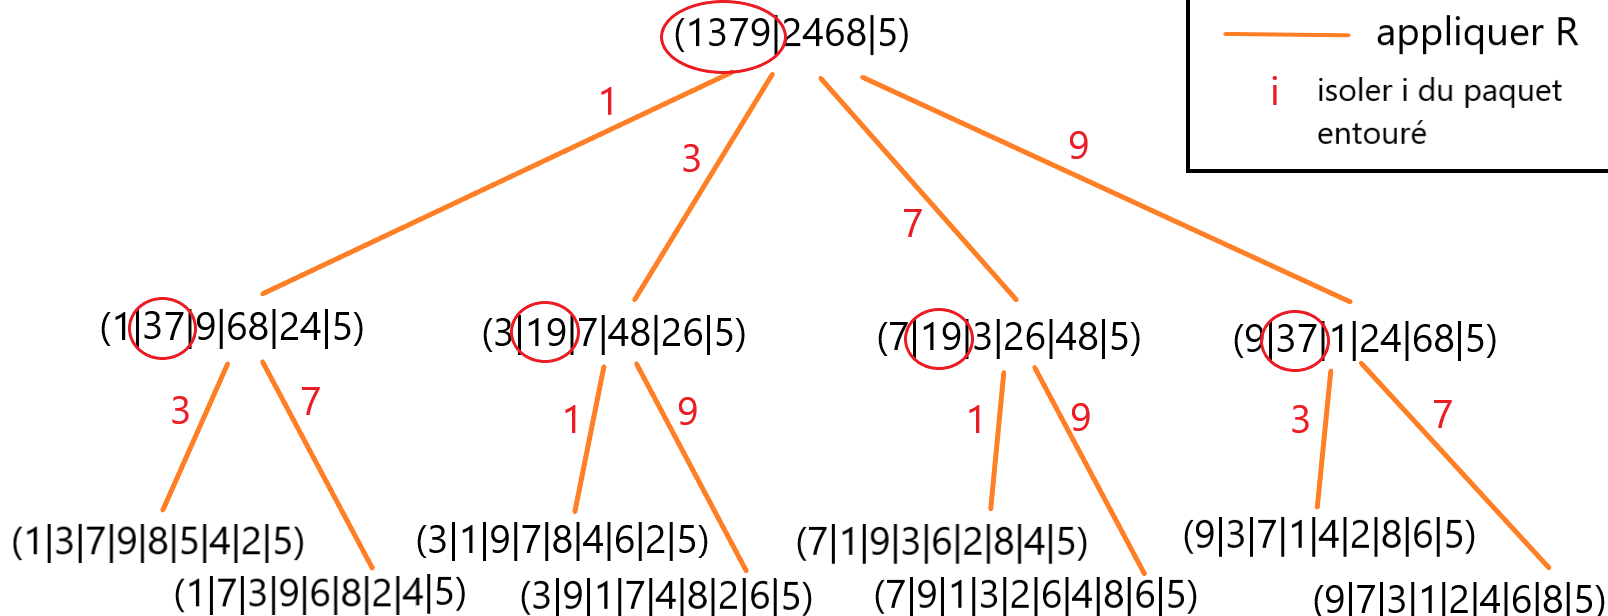
\includegraphics[width = 8.5cm]{search_tree}
    \caption{\label{fig:Arbre T(G)} Arbre T(G) de racine $\pi=(1\ 3\ 7\ 9\ |\ 2\ 4\ 6\ 8\ |\ 5)$}
\end{figure}

\subsection{Isomorphisme canonique \cite{mckay_label}}
\noindent \underline{Ordre total $\preceq$ sur les graphes} : \newline \newline
On pose la fonction $i:\ G\ \longmapsto i(G)$ telle que : \newline
$\quad \bullet \ i(G)$ est la séquence binaire $(\mathds{1}_{(i,j)\in G})$ avec $(i,j)$ dans l'ordre lexicographique \newline
$\quad \bullet \ G \preceq H$ si et seulement si $i(G) \leq i(H)$ en décimal
\newline \newline
On pose alors l'\textbf{ismorphisme canonique de McKay} (pour le tri $\pi$):
\begin{equation}
    \boxed{C_M(G) = max_{\preceq}\ \lbrace G^{\sigma},\ \sigma \text{ noeud terminal de T(G) de racine } \pi \rbrace }
\end{equation}
alors:
\begin{equation}
    \boxed{G \cong H \text{ si et seulement si } C_M(G) = C_M(H)}
\end{equation}
\newline
\noindent \underline{Exemple} : pour $\pi = (1\ |\ 3\ 7\ |\ 9\ |\ 6\ 8\ |\ 2\ 4\ |\ 5)$

\begin{multicols}{2}
    \begin{figure}[H]
        \centering
        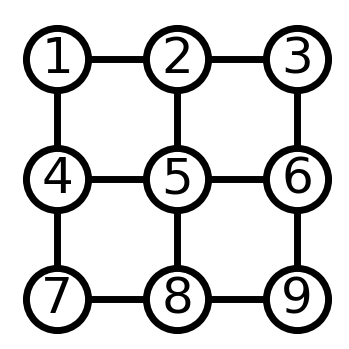
\includegraphics[width = 2.4cm]{graph_tri_equal}
        \caption{\label{fig: Graphe G}Graphe G}
    \end{figure}
    \vfill
    \begin{figure}[H]
        \centering
        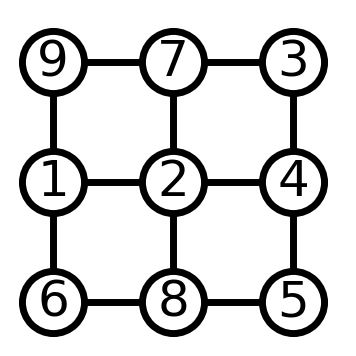
\includegraphics[width = 2.4cm]{cmg}
        \caption{\label{fig: Isomorphe G} Graphe $C_M(G)$}
    \end{figure}
\end{multicols}

\section{Plus grand sous-graphe isomorphe commun}
\subsection{Choix de la méthode utilisée pour le test d'ismorphisme sur deux sous-graphes}
Dans le cas particulier des protéines, le tri équitable (tri le plus fin obtenu par propagation du degré) proposé par McKay est très efficace et produit des paquets de très petite taille.
En combinant ce tri et le test d'isomorphisme sur les graphes à sommets triés, on obtient un algorithme très efficace, plus efficace que la méthode complète de McKay. \newline

\noindent \underline{Exemple} : 
\begin{multicols}{2}
    \begin{figure}[H]
        \centering
        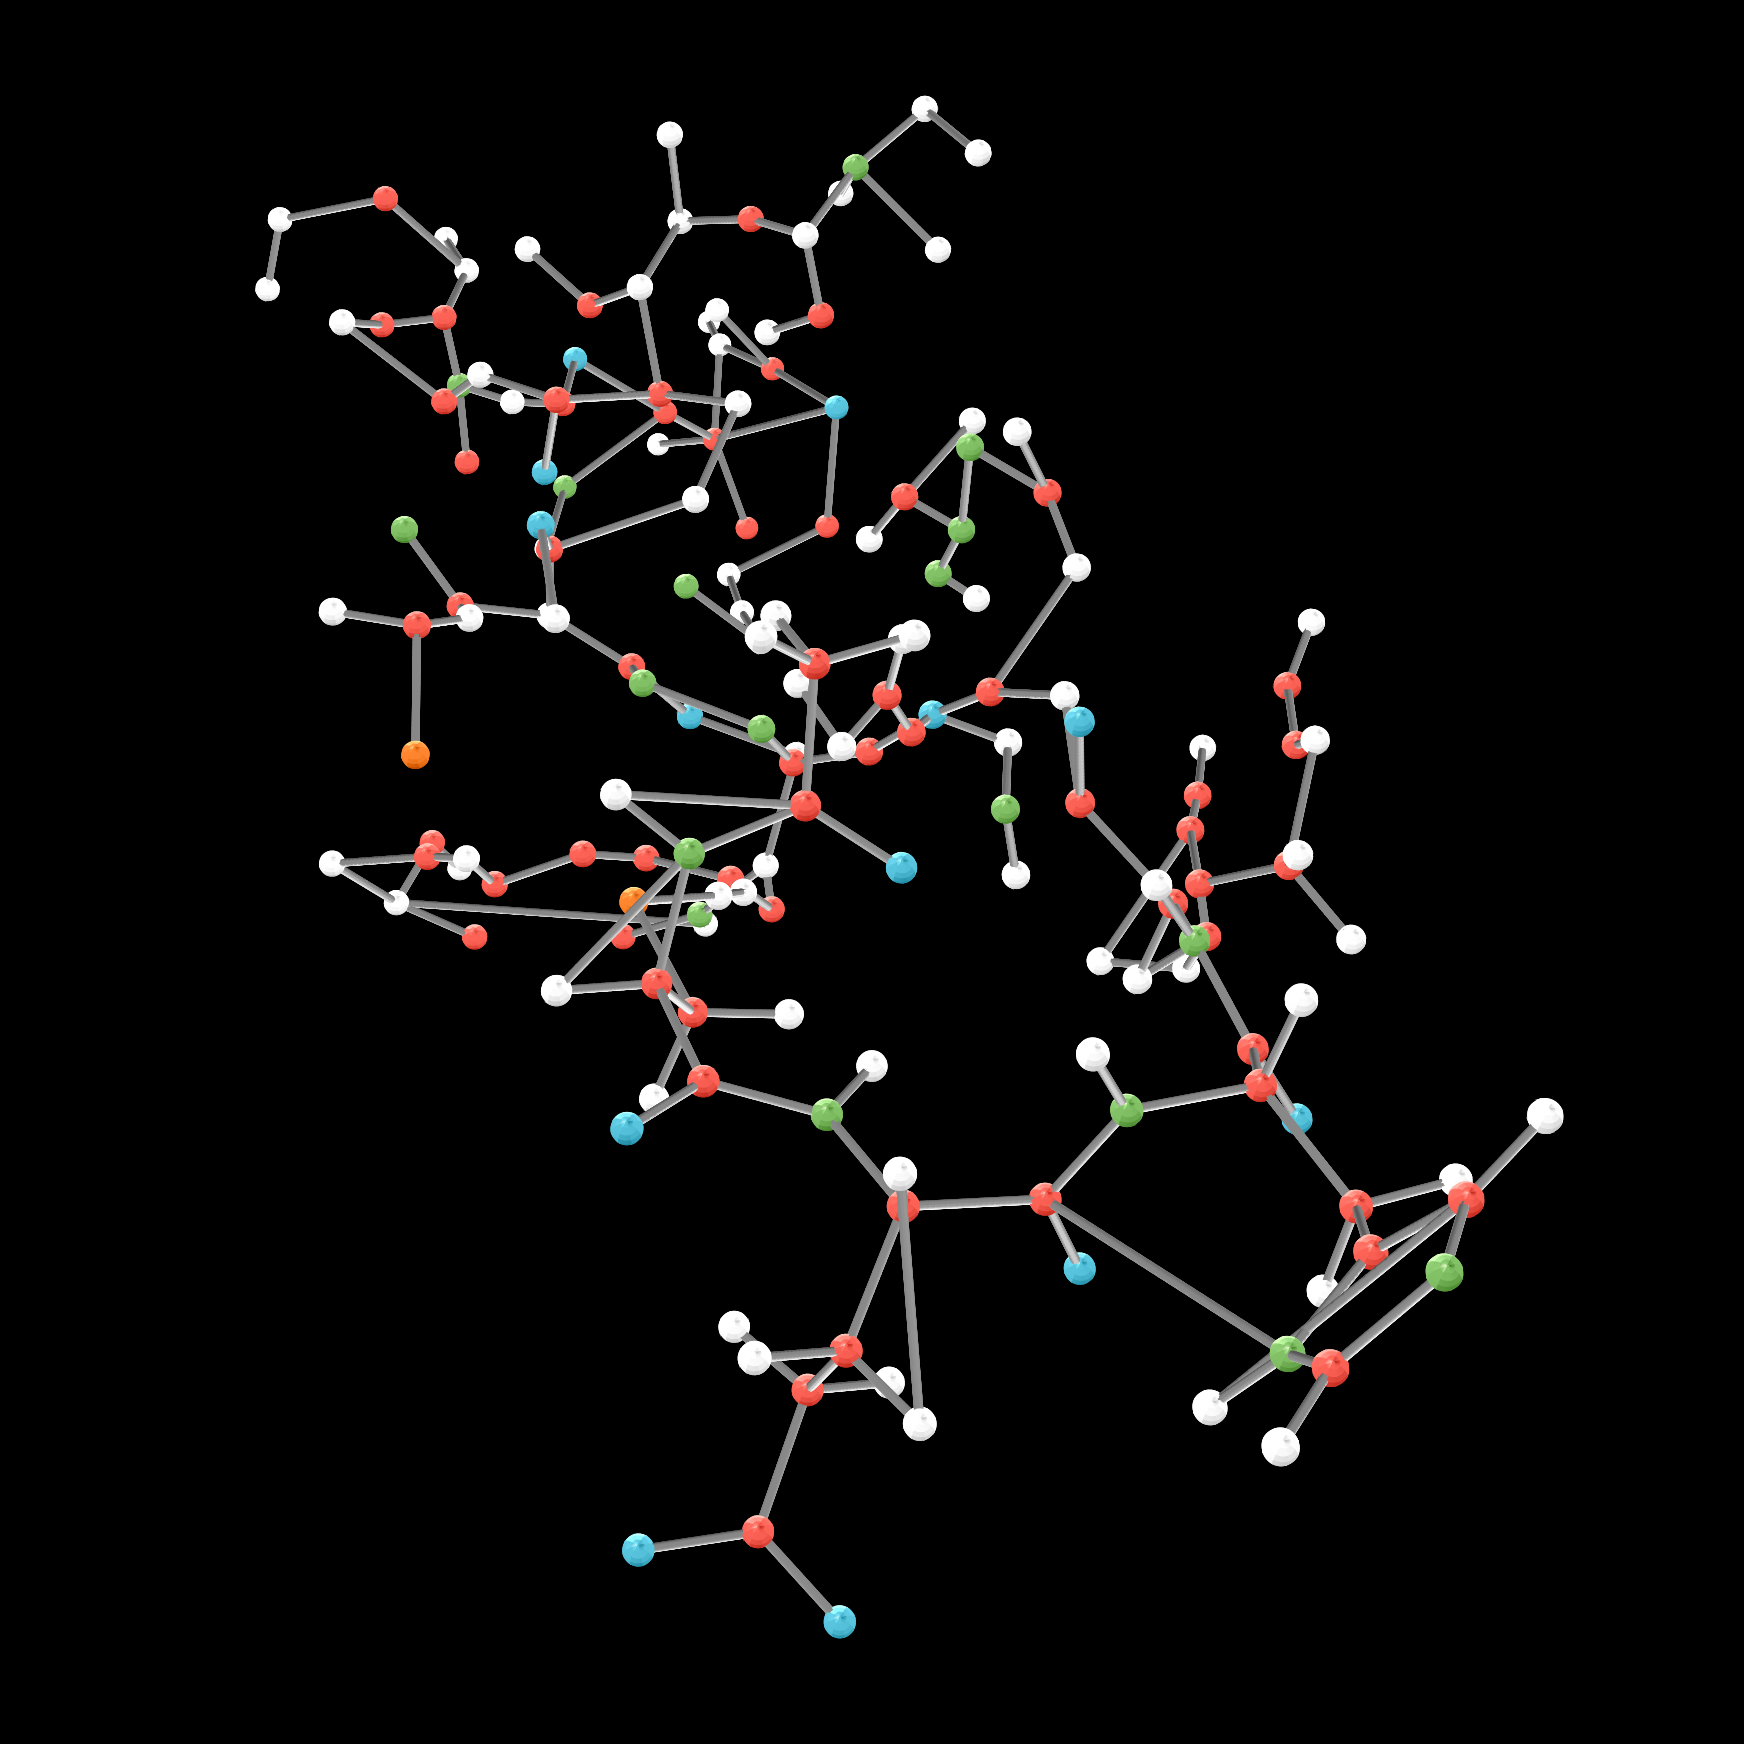
\includegraphics[width = 5cm]{protein_cov}
        \caption{\label{fig: Protéine}Protéine}
    \end{figure}
    \begin{center}
    \begin{figure}[H]
        \centering
        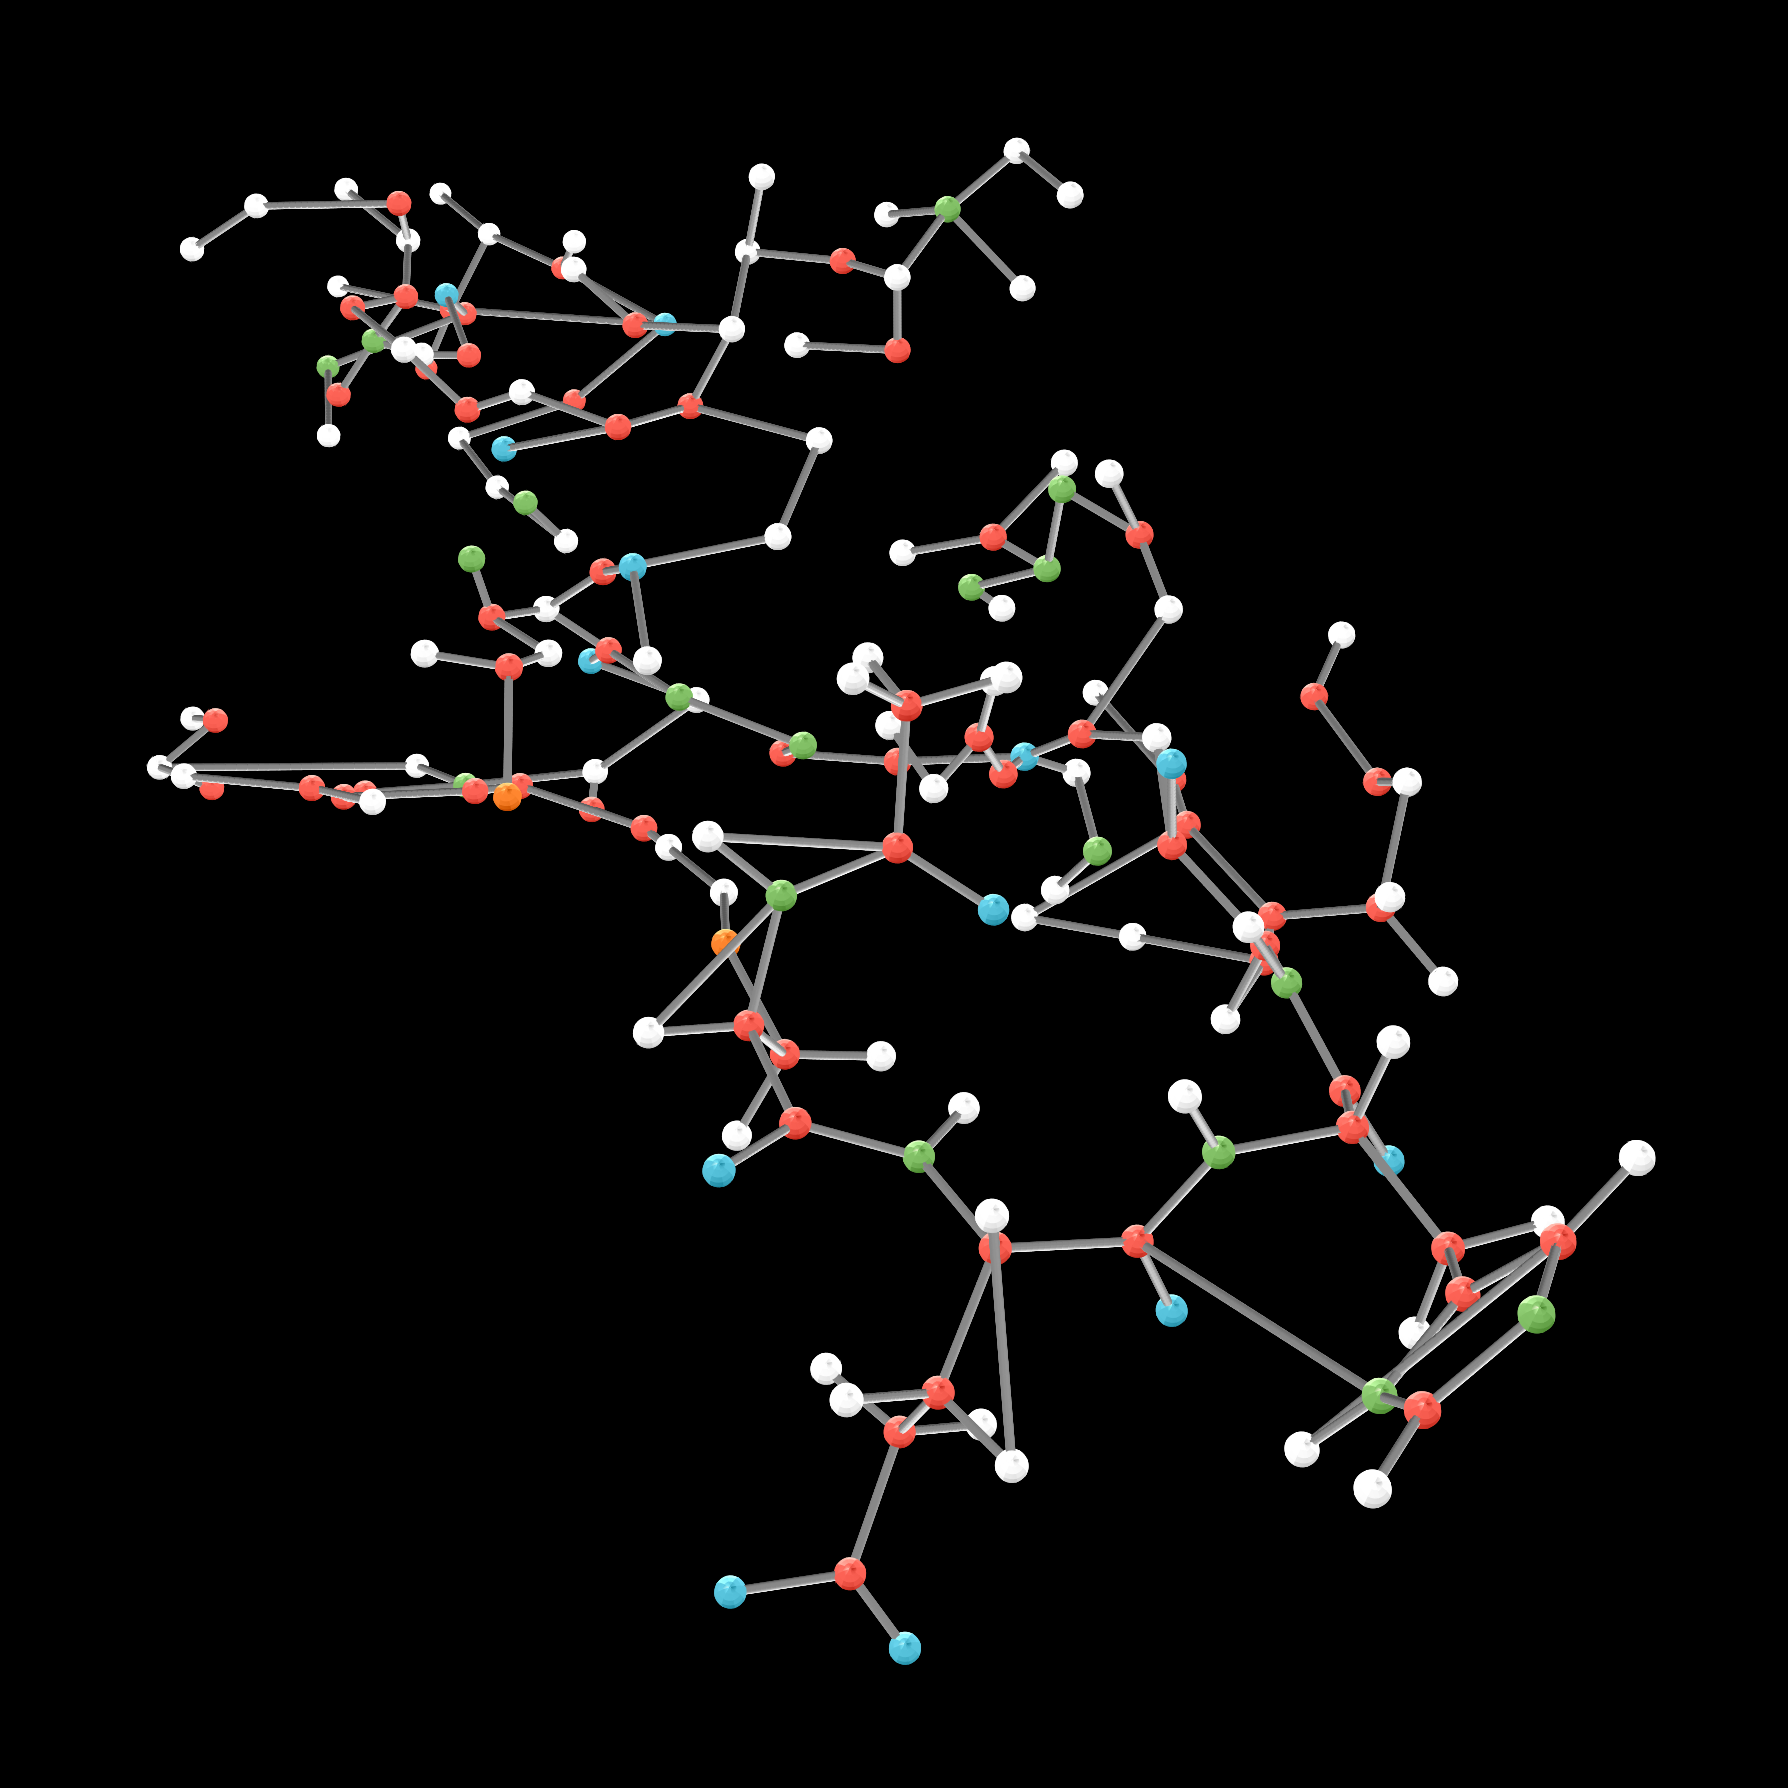
\includegraphics[width = 5cm]{protein_cov_translatee}
        \caption{\label{fig: Proteine translatee}Même protéine mais déplacée et numérotation différente des sommets}
    \end{figure}
\end{center}
\end{multicols}
\underline{Temps d'éxecution} : pour cette protéine de 171 atomes
\begin{center}
\begin{tabular}{c|c}
    tri par degré et atomes & 0.002 s\\
    propagation des degrés & 7.4 s \\
    test d'isomorphisme & 0.3 s \\
    temps total d'éxecution & 7.8 s
\end{tabular}
\end{center}

\subsection{Itération sur les sous-graphes}
\noindent On cherche la sous-structure de taille maximale de $G_1=A_1\times S_1$ et $G_2=A_2\times S_2$ :
\begin{itemize}
    \item itération pour k allant de min($|S_1|$,$|S_2|$) à 1 (sur le nombre d'arêtes du sous-graphe)
    \item pour un sous-graphe de k arêtes, on itère sur l'ensemble de parties de k arêtes de $G_1$ formant un graphe connexe
    \item pour un sous-graphe donné de $G_1$ de k arêtes, on itère sur l'ensemble de parties de k arêtes de $G_2$ formant un graphe connexe
    \item test d'isomorphsime sur les sous-graphes de k arêtes
\end{itemize}
\underline{Complexité en nombre de tests d'isomorphismes} : exponentielle , en $O( 4^{min(|S_1|,|S_2|)})$
mais beaucoup de cas sont écartés rapidement, si les sous-graphes ne sont pas connexes ou les tris formés de tailles différentes \newline

\noindent \underline{NB} : on peut trouver plusieurs sous-graphes isomorphes de taille maximale \newline
Comment choisir parmi ces sous-structures isomorphes ?

\subsection{Cas d'égalité}
L'idée est de comparer comment les structures sont formées dans l'espace.

\section{Comparaison des positions de structures isomorphes}
\subsection{Application du coefficient des branches sur les structures}
Il exite une bijection entre les arêtes des strcutures comparées (on les suppose isomorphes).
Il est alors possible d'utiliser le même coefficient de comparaison que pour les branches,
après alignement, en ordonnant les arêtes des structures.

\section{Comparaison de protéines}
\subsection{Coefficient de comparaison}
L'idée est d'associer à deux protéines données un coefficient de comparaison C$\in [0,100]$ selon deux paramètres :
\begin{itemize}
    \item la taille des plus grandes sous-structures isomorphes :
    $C_{struct} = \frac{\text{taille sous-struct}}{\text{taille moyenne des 2 protéines}}$ \newline
    \item la proximité dans l'espace des deux plus grandes sous-structures isomorphes : 
    $C_{prox}$ est le coefficient de comparaison de branches mais appliqué sur les arêtes des sous-structures isomorphes
\end{itemize}
alors $\boxed{C = \displaystyle \frac{C_{prox}+C_{struct}}{2}}$

\subsection{Exemples de coefficients de comparaison de protéines}
\begin{multicols}{2}
    \begin{figure}[H]
        \centering
        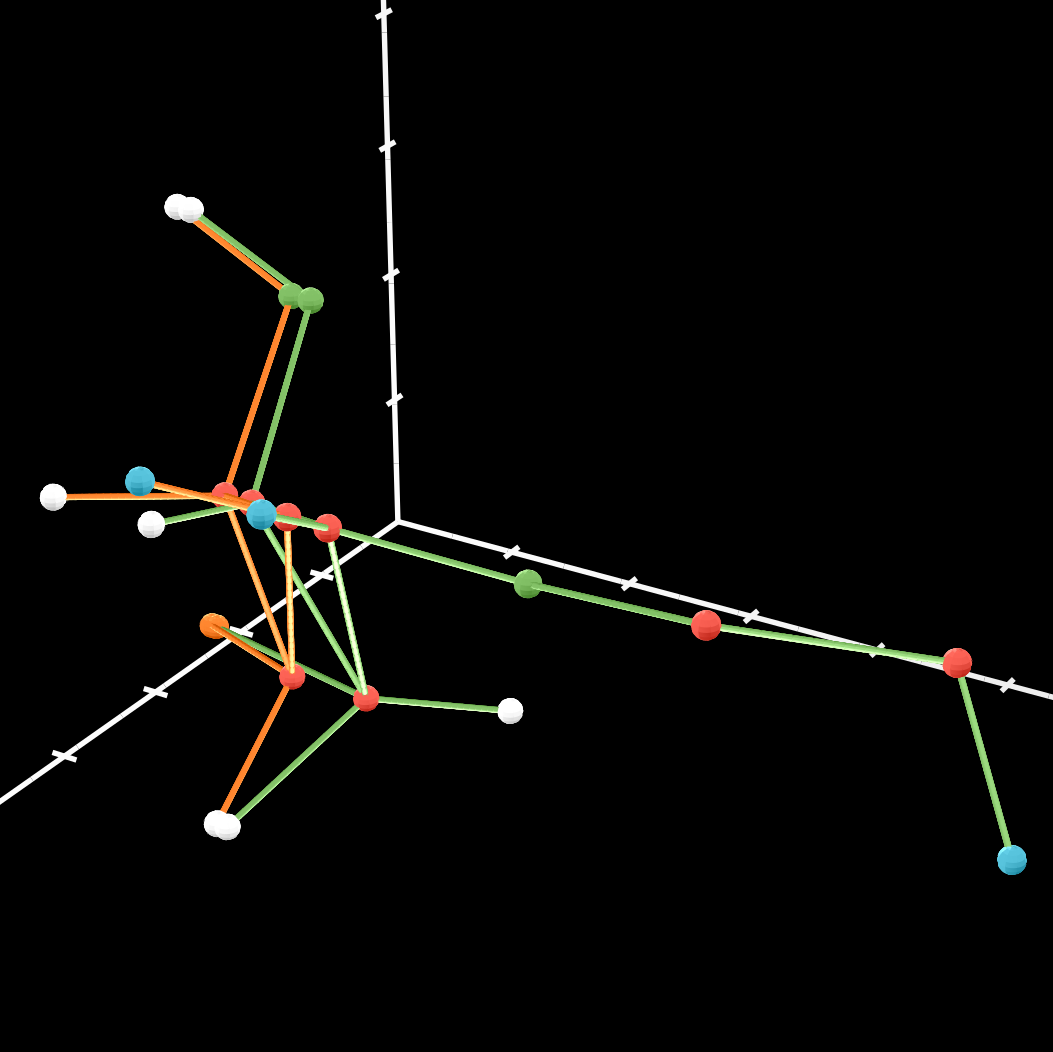
\includegraphics[width = 4cm]{comp_sub_loin}
        \caption{\label{fig: subcomp_loin} Protéines plutôt éloignées}
    \end{figure}
    \begin{figure}[H]
        \centering
        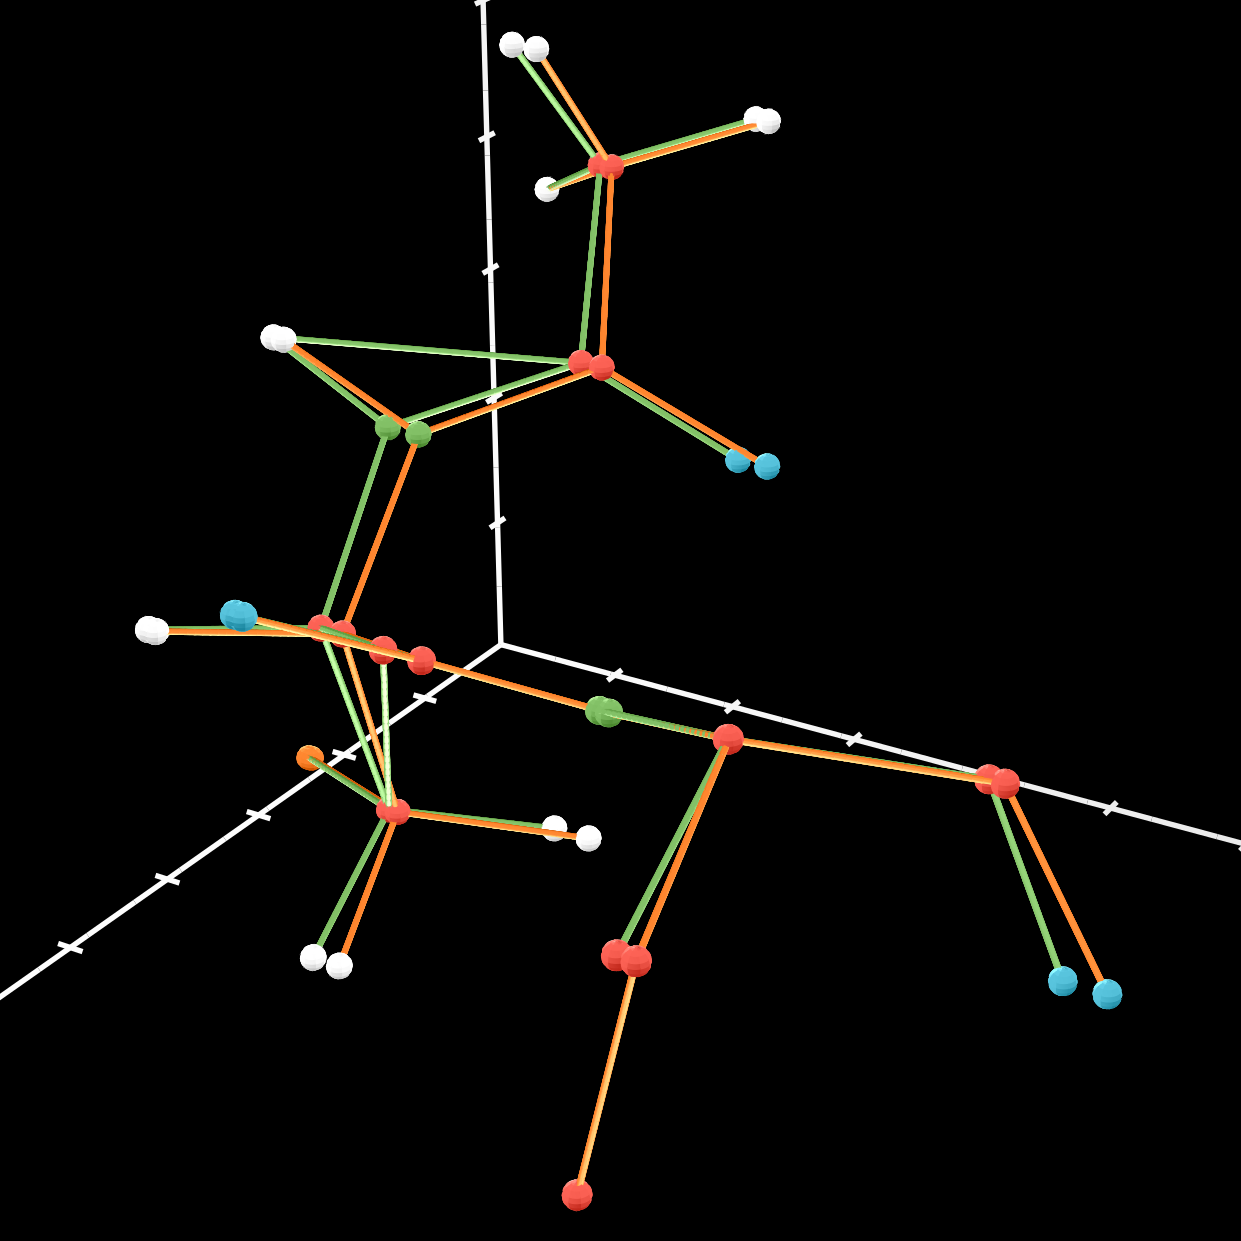
\includegraphics[width = 4cm]{comp_sub_proche}
        \caption{\label{fig: subcom_proche} Protéines plutôt proches}
    \end{figure}
\end{multicols}

\begin{multicols}{2}
    \begin{center}
        $C_{prox}=92.9 \qquad C_{struct}=52$\newline \newline
        $\boxed{C=72}$
    \end{center}
    \begin{center}
        $C_{prox}=97.7 \qquad C_{struct}=93$\newline \newline
        $\boxed{C=95}$
    \end{center}
\end{multicols}

\begin{thebibliography}{2} 
    \bibitem[1]{mckay_label} Stephen G. Hartke and A. J. Radcliffe, McKay's Canonical Graph labeling algorithm, 2008 
    \bibitem[2]{mckay} Brendan D. McKay, Pratical Graph Isomorphism, 1981
    \bibitem[3]{pdb} Base de données PDB, https://www.rcsb.org/
\end{thebibliography}

\end{document}
